\section{Factorieel en OFAT-onderzoek}
\label{app:meta}

\begingroup
\footnotesize
\setlength{\tabcolsep}{2.5pt}
\setlength{\intextsep}{5pt}
\setlength{\abovecaptionskip}{3pt}
\setlength{\belowcaptionskip}{2pt}
\renewcommand{\arraystretch}{0.96}

\begin{table}[H]
\centering
\caption{Volledig $2\times2\times2$-SA-ontwerp met een capaciteitsvullende
randomstart. Voor elke seed zijn $D$ en de interne solvertijd over de twaalf
waves opgeteld. De resultaten zijn gebaseerd op tien gekoppelde seeds.}
\label{tab:app-sa}
\begin{tabular}{@{}lllrrr@{}}
\toprule
\textbf{start} & \textbf{koeling} & \textbf{buurt} &
\textbf{$\bar D\pm$SD} & \textbf{beste $D$} & \textbf{$\bar t$ (s)} \\
\midrule
greedy & geometrisch & relocate & $5\,308\,303\pm458$ & $5\,307\,359$ & $12,179$ \\
greedy & geometrisch & swap     & $5\,307\,697\pm527$ & $5\,306\,678$ & $12,219$ \\
greedy & Lundy--Mees & relocate & $5\,308\,154\pm441$ & $5\,307\,423$ & $13,174$ \\
greedy & Lundy--Mees & swap     & $5\,307\,592\pm450$ & $5\,306\,974$ & $12,079$ \\
\midrule
willekeurig & geometrisch & relocate & $10\,956\,014\pm22\,702$ & $10\,917\,264$ & $0,028$ \\
willekeurig & geometrisch & swap     & $10\,562\,728\pm18\,863$ & $10\,538\,780$ & $0,027$ \\
willekeurig & Lundy--Mees & relocate & $10\,970\,186\pm8\,831$  & $10\,957\,547$ & $0,027$ \\
willekeurig & Lundy--Mees & swap     & $10\,545\,832\pm29\,989$ & $10\,501\,489$ & $0,028$ \\
\bottomrule
\end{tabular}
\end{table}

\begin{table}[H]
\centering
\caption{Gekoppelde SA-effecten op $D$. De Student-$t$-95\%-BI's zijn
ongecorrigeerd. De kolom $p_{\mathrm H}$ bevat de Holm-gecorrigeerde $p$-waarden voor
zeven toetsen. De contrasten zijn $K$: Lundy--Mees min geometrisch, $B$: swap
min relocate en $S$: willekeurig min greedy. Een positieve $\Delta D$ is
ongunstig.}
\label{tab:app-sa-effects}
\begin{tabular}{@{}lrr@{}}
\toprule
\textbf{effect} & \textbf{$\Delta D$ [95\%-BI]} & \textbf{$p_{\mathrm H}$} \\
\midrule
$K$             & $-744\;[-9\,200\text{--}7\,712]$ & $1,000$ \\
$B$             & $-204\,702\;[-211\,956\text{--}-197\,448]$ & $1,68\!\cdot\!10^{-12}$ \\
$S$             & $+5\,450\,754\;[5\,442\,863\text{--}5\,458\,644]$ & $6,41\!\cdot\!10^{-25}$ \\
$K\times B$     & $-15\,511\;[-29\,477\text{--}-1\,545]$ & $0,133$ \\
$K\times S$     & $-1\,235\;[-18\,181\text{--}15\,711]$ & $1,000$ \\
$B\times S$     & $-408\,236\;[-422\,662\text{--}-393\,810]$ & $1,68\!\cdot\!10^{-12}$ \\
$K\times B\times S$ & $-31\,112\;[-59\,457\text{--}-2\,766]$ & $0,133$ \\
\bottomrule
\end{tabular}
\end{table}

\begin{table}[H]
\centering
\caption{Gekoppelde GA-OFAT-contrasten. Elke rij geeft het verschil tussen de
variant en de basis met populatie 12, twintig generaties, mutatiekans 0,20 en
elitisme 0,08. De Student-$t$-95\%-BI's zijn ongecorrigeerd. De kolom
$p_{\mathrm H}$ bevat de Holm-gecorrigeerde $p$-waarden voor acht kwaliteitstoetsen.}
\label{tab:app-ga}
\begin{tabular}{@{}llrrr@{}}
\toprule
\textbf{factor} & \textbf{variant (basis)} & \textbf{$\Delta D$ [95\%-BI]} &
\textbf{$p_{\mathrm H}$} & \textbf{$\Delta t$} \\
\midrule
populatie  & 6 (12)       & $+48\;[-83\text{--}180]$    & $1,000$ & $-26,32\%$ \\
populatie  & 24 (12)      & $-243\;[-478\text{--}-9]$   & $0,347$ & $+55,25\%$ \\
generaties & 10 (20)      & $+81\;[-13\text{--}175]$    & $0,589$ & $-15,21\%$ \\
generaties & 40 (20)      & $-54\;[-230\text{--}122]$   & $1,000$ & $+21,29\%$ \\
mutatiekans & 0,05 (0,20) & $+48\;[-85\text{--}180]$    & $1,000$ & $-2,86\%$ \\
mutatiekans & 0,40 (0,20) & $-39\;[-194\text{--}115]$   & $1,000$ & $+0,61\%$ \\
elitisme   & 0 (0,08)     & $+49\;[-81\text{--}179]$    & $1,000$ & $+17,31\%$ \\
elitisme   & 0,20 (0,08)  & $-13\;[-188\text{--}163]$   & $1,000$ & $-5,76\%$ \\
\bottomrule
\end{tabular}
\end{table}

\noindent De OFAT-resultaten gelden alleen voor OX, toernooigrootte 3 en een
50/50-verdeling van invoeg- en wisselmutaties. Door afronding gebruiken
populaties van 6, 12 en 24 respectievelijk 0, 1 en 2 elites. Het effect van de
populatiegrootte kan daardoor niet van het aantal elites worden gescheiden.
Omdat de uitvoeringsvolgorde niet was gerandomiseerd, zijn de tijdsverschillen
uitsluitend beschrijvend.
\endgroup

\clearpage
\section{Budget, schaalgedrag, waveverschillen en convergentie}
\label{app:matched}

\begingroup
\footnotesize
\setlength{\tabcolsep}{2.2pt}
\setlength{\intextsep}{5pt}
\setlength{\abovecaptionskip}{3pt}
\setlength{\belowcaptionskip}{2pt}
\renewcommand{\arraystretch}{0.94}

\begin{table}[H]
\centering
\caption{Afzonderlijke Release-budgetstudie met tien gekoppelde seeds. Per seed
zijn $D$ en de interne solvertijd over twaalf waves opgeteld. Winst is berekend
als de greedyscore min de kandidaatscore, zodat een positieve waarde een
verbetering aangeeft. De Student-$t$-95\%-BI's zijn ongecorrigeerd. De kolom
$p_{\mathrm H}$ bevat de Holm-gecorrigeerde $p$-waarden voor zeven budgettoetsen.}
\label{tab:app-budget}
\begin{tabular}{@{}lrrrr@{}}
\toprule
\textbf{configuratie} & \textbf{$\bar D\pm$SD} & \textbf{$\bar t\pm$SD (s)} &
\textbf{winst in \% [95\%-BI]} & \textbf{$p_{\mathrm H}$} \\
\midrule
greedy       & $5\,307\,302\pm0$      & $12,057\pm0,367$ & $0$ & --- \\
SA--120      & $5\,307\,102\pm275$    & $12,876\pm1,912$ & $0,0038\;[0,0001\text{--}0,0075]$ & $0,141$ \\
SA--400      & $5\,307\,048\pm248$    & $12,016\pm0,233$ & $0,0048\;[0,0014\text{--}0,0081]$ & $0,0413$ \\
SA--2\,000  & $5\,306\,260\pm602$    & $12,521\pm0,655$ & $0,0196\;[0,0115\text{--}0,0278]$ & $0,00235$ \\
SA--10\,000 & $5\,301\,464\pm1\,789$ & $13,195\pm0,555$ & $0,1100\;[0,0859\text{--}0,1341]$ & $1,93\!\cdot\!10^{-5}$ \\
GA--10       & $5\,307\,299\pm9$      & $21,549\pm1,942$ & $0,0001\;[-0,0001\text{--}0,0002]$ & $0,290$ \\
GA--20       & $5\,307\,171\pm211$    & $24,353\pm0,744$ & $0,0025\;[-0,0004\text{--}0,0053]$ & $0,161$ \\
GA--40       & $5\,307\,044\pm182$    & $31,148\pm1,823$ & $0,0049\;[0,0024\text{--}0,0073]$ & $0,00751$ \\
\bottomrule
\end{tabular}
\end{table}

\begin{table}[H]
\centering
\caption{De exponent $b$ is met een log--logregressie van $T(n)=a n^b$ geschat
op vijf groottes en negen timings per grootte. Het Student-$t$-95\%-BI voor $b$
heeft drie vrijheidsgraden. De fit geldt alleen voor $50\leq n\leq800$.}
\label{tab:app-scaling}
\begin{tabular}{@{}lrrr@{}}
\toprule
\textbf{methode} & \textbf{$b$ [95\%-BI]} & \textbf{$R^2$} &
\textbf{mediaan $t_{800}$ (ms)} \\
\midrule
greedy & $1,888\;[1,810\text{--}1,967]$ & $0,9995$ & $648,16$ \\
SA     & $1,892\;[1,842\text{--}1,942]$ & $0,9998$ & $638,49$ \\
GA     & $1,303\;[1,176\text{--}1,429]$ & $0,9972$ & $1\,442,14$ \\
\bottomrule
\end{tabular}
\end{table}

\begin{table}[H]
\centering
\caption{De vier waves met Holm-significante winst voor SA--10\,000. Correctie
gebeurt over alle twaalf wave-toetsen.}
\label{tab:app-waves}
\begin{tabular}{@{}rrrrr@{}}
\toprule
\textbf{wave} & \textbf{orders} & \textbf{winst $D$ [95\%-BI]} &
\textbf{winst (\%)} & \textbf{$p_{\mathrm H}$} \\
\midrule
02 & $1\,076$ & $270\;[142\text{--}397]$       & $0,0385$ & $0,0101$ \\
05 & $909$     & $1\,260\;[647\text{--}1\,873]$ & $0,2814$ & $0,0109$ \\
07 & $974$     & $445\;[313\text{--}577]$       & $0,0647$ & $0,000365$ \\
10 & $858$     & $1\,220\;[1\,017\text{--}1\,424]$ & $0,1783$ & $3,27\!\cdot\!10^{-6}$ \\
\bottomrule
\end{tabular}
\end{table}

\noindent Bij GA--40 verbetert minstens één seed in vijf van de twaalf waves.
Geen enkele wave heeft een positief ongecorrigeerd 95\%-BI of blijft na
Holm-correctie significant.

\begin{table}[H]
\centering
\caption{Lange convergentiestudie met tien seeds per budget. $t_{95}$ en
$t_{99}$ zijn berekend binnen het eigen budget en alleen voor runs die
verbeteren. De laatste kolom telt achtereenvolgens runs zonder winst, runs met
winst in de laatste 10\% en runs met winst op de eindstap.}
\label{tab:app-convergence}
\begin{tabular}{@{}lrrrrr@{}}
\toprule
\textbf{config.} & \textbf{$\bar D\pm$SD} & \textbf{$\bar t$ (s)} &
\textbf{$t_{95}$ [IQR]} & \textbf{$t_{99}$ [IQR]} &
\textbf{geen/laat/einde} \\
\midrule
SA--10\,000 & $5\,302\,372\pm1\,221$ & $13,793$ & $9\,259\;[8\,598\text{--}9\,339]$ & $9\,415\;[9\,256\text{--}9\,594]$ & $0/10/0$ \\
SA--50\,000 & $5\,288\,766\pm1\,436$ & $16,302$ & $42\,872\;[41\,143\text{--}46\,000]$ & $47\,924\;[46\,263\text{--}49\,191]$ & $0/10/0$ \\
GA--40  & $5\,308\,482\pm206$ & $32,315$ & $28\;[18\text{--}39]$ & $28\;[18\text{--}39]$ & $5/2/1$ \\
GA--100 & $5\,308\,043\pm482$ & $53,373$ & $83\;[75\text{--}90]$ & $84\;[82\text{--}92]$ & $1/4/1$ \\
GA--200 & $5\,307\,506\pm793$ & $88,876$ & $164\;[145\text{--}172]$ & $164\;[145\text{--}172]$ & $1/1/0$ \\
\bottomrule
\end{tabular}
\end{table}

\endgroup

\clearpage
\section{Constructieregels en greedy-ontwikkeling}
\label{app:heuristics}

\begingroup
\footnotesize
\setlength{\tabcolsep}{2.7pt}
\setlength{\intextsep}{5pt}
\setlength{\abovecaptionskip}{3pt}
\setlength{\belowcaptionskip}{2pt}
\renewcommand{\arraystretch}{0.96}

\begin{table}[H]
\centering
\caption{Veertien deterministische varianten van seedregel, selectieregel en
$K$. De tien procesuitvoeringen van elke configuratie leverden exact dezelfde
doelfunctiewaarde op. De laatste kolom toont de mediane tijd en IQR uit een
gerandomiseerde uitvoeringsvolgorde.}
\label{tab:app-seed}
\begin{tabular}{@{}llcrr@{}}
\toprule
\textbf{seed} & \textbf{selectie} & \textbf{$K$} & \textbf{$D$} &
\textbf{interne tijd (s)} \\
\midrule
grootste span & locatieoverlap       & --- & $7\,485\,444$ & $7,146\;[6,700\text{--}7,285]$ \\
grootste span & spanuitbreiding      & --- & $6\,759\,161$ & $6,681\;[6,630\text{--}6,834]$ \\
grootste span & incrementele kost    & --- & $6\,566\,051$ & $6,917\;[6,768\text{--}7,573]$ \\
grootste span & tweestapsvooruitblik & 2   & $6\,506\,732$ & $12,659\;[12,412\text{--}13,099]$ \\
grootste span & tweestapsvooruitblik & 4   & $6\,517\,269$ & $24,034\;[23,031\text{--}27,302]$ \\
grootste span & tweestapsvooruitblik & 8   & $6\,491\,675$ & $42,355\;[41,281\text{--}44,547]$ \\
grootste span & tweestapsvooruitblik & 16  & $6\,492\,775$ & $77,783\;[77,011\text{--}82,117]$ \\
\midrule
kleinste span & locatieoverlap       & --- & $7\,722\,909$ & $6,850\;[6,692\text{--}7,115]$ \\
kleinste span & spanuitbreiding      & --- & $6\,836\,623$ & $6,705\;[6,629\text{--}6,743]$ \\
kleinste span & incrementele kost    & --- & $5\,487\,174$ & $6,880\;[6,748\text{--}7,344]$ \\
kleinste span & tweestapsvooruitblik & 2   & $5\,486\,876$ & $12,744\;[12,471\text{--}13,855]$ \\
kleinste span & tweestapsvooruitblik & 4   & $5\,441\,472$ & $22,074\;[21,803\text{--}22,413]$ \\
kleinste span & tweestapsvooruitblik & 8   & $5\,436\,249$ & $41,075\;[40,377\text{--}41,421]$ \\
kleinste span & tweestapsvooruitblik & 16  & $5\,447\,494$ & $77,380\;[76,707\text{--}78,402]$ \\
\bottomrule
\end{tabular}
\end{table}

\begin{table}[H]
\centering
\caption{Zeven opeenvolgende mijlpalen in de adaptieve greedy-ontwikkeling. De
marginale winst is telkens het verschil met de voorgaande samengestelde
configuratie. De historische tijden zijn afgeronde enkelvoudige metingen.}
\label{tab:app-greedy}
\begin{tabular}{@{}lrrrr@{}}
\toprule
\textbf{cumulatieve configuratie} & \textbf{$D$} &
\textbf{marginale winst} & \textbf{routes} & \textbf{hist. tijd (s)} \\
\midrule
besparingsbasis                 & $5\,511\,080$ & ---       & 534 & 20 \\
$+$ lokale paarzoektocht        & $5\,100\,290$ & $410\,790$ & 534 & 81 \\
$+$ eliminatie en post-LS       & $5\,066\,010$ & $34\,280$  & 517 & 135 \\
$+$ paarheropbouw en afsluitende LS & $5\,002\,250$ & $63\,760$  & 517 & 487 \\
$+$ routedrietalheropbouw       & $4\,996\,960$ & $5\,290$   & 517 & 565 \\
$+$ drietalcyclus en combinatievenster & $4\,944\,950$ & $52\,010$ & 517 & $2\,383$ \\
$+$ afsluitende paarheropbouw   & $4\,941\,530$ & $3\,420$   & 517 & $2\,523$ \\
\bottomrule
\end{tabular}
\end{table}

\noindent Over het volledige ontwikkelingspad daalt $D$ met $569\,550$
($10,335\%$). Omdat alle mechanismen op dezelfde instantie zijn ontwikkeld en
geselecteerd, kunnen de resultaten zonder afzonderlijke testinstantie niet
worden veralgemeend.

\begin{figure}[H]
\centering
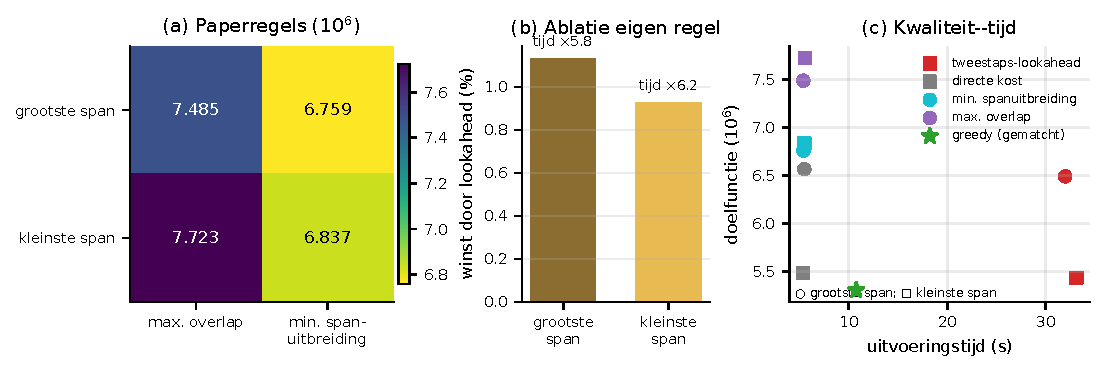
\includegraphics[width=0.82\linewidth]{figures/retrospective_seed.pdf}
\caption{De drie panelen tonen de doelfunctie van het oorspronkelijke
$2\times2$-ontwerp, de winst van de tweestapsvooruitblik en de mediane tijd met
IQR uit tien procesmetingen.}
\label{fig:app-seed}
\end{figure}
\endgroup
